
%% bare_conf.tex
%% V1.4b
%% 2015/08/26
%% by Michael Shell
%% See:
%% http://www.michaelshell.org/
%% for current contact information.
%%
%% This is a skeleton file demonstrating the use of IEEEtran.cls
%% (requires IEEEtran.cls version 1.8b or later) with an IEEE
%% conference paper.
%%
%% Support sites:
%% http://www.michaelshell.org/tex/ieeetran/
%% http://www.ctan.org/pkg/ieeetran
%% and
%% http://www.ieee.org/

%%*************************************************************************
%% Legal Notice:
%% This code is offered as-is without any warranty either expressed or
%% implied; without even the implied warranty of MERCHANTABILITY or
%% FITNESS FOR A PARTICULAR PURPOSE!
%% User assumes all risk.
%% In no event shall the IEEE or any contributor to this code be liable for
%% any damages or losses, including, but not limited to, incidental,
%% consequential, or any other damages, resulting from the use or misuse
%% of any information contained here.
%%
%% All comments are the opinions of their respective authors and are not
%% necessarily endorsed by the IEEE.
%%
%% This work is distributed under the LaTeX Project Public License (LPPL)
%% ( http://www.latex-project.org/ ) version 1.3, and may be freely used,
%% distributed and modified. A copy of the LPPL, version 1.3, is included
%% in the base LaTeX documentation of all distributions of LaTeX released
%% 2003/12/01 or later.
%% Retain all contribution notices and credits.
%% ** Modified files should be clearly indicated as such, including  **
%% ** renaming them and changing author support contact information. **
%%*************************************************************************


% *** Authors should verify (and, if needed, correct) their LaTeX system  ***
% *** with the testflow diagnostic prior to trusting their LaTeX platform ***
% *** with production work. The IEEE's font choices and paper sizes can   ***
% *** trigger bugs that do not appear when using other class files.       ***                          ***
% The testflow support page is at:
% http://www.michaelshell.org/tex/testflow/



\documentclass[conference]{IEEEtran}
% Some Computer Society conferences also require the compsoc mode option,
% but others use the standard conference format.
%
% If IEEEtran.cls has not been installed into the LaTeX system files,
% manually specify the path to it like:
% \documentclass[conference]{../sty/IEEEtran}




\usepackage{amsmath}
\usepackage{graphicx}

\DeclareMathOperator{\Tr}{Tr}
% Some very useful LaTeX packages include:
% (uncomment the ones you want to load)


% *** MISC UTILITY PACKAGES ***
%
%\usepackage{ifpdf}
% Heiko Oberdiek's ifpdf.sty is very useful if you need conditional
% compilation based on whether the output is pdf or dvi.
% usage:
% \ifpdf
%   % pdf code
% \else
%   % dvi code
% \fi
% The latest version of ifpdf.sty can be obtained from:
% http://www.ctan.org/pkg/ifpdf
% Also, note that IEEEtran.cls V1.7 and later provides a builtin
% \ifCLASSINFOpdf conditional that works the same way.
% When switching from latex to pdflatex and vice-versa, the compiler may
% have to be run twice to clear warning/error messages.





\usepackage{hyperref}
% *** CITATION PACKAGES ***
%
\usepackage{cite}
% cite.sty was written by Donald Arseneau
% V1.6 and later of IEEEtran pre-defines the format of the cite.sty package
% \cite{} output to follow that of the IEEE. Loading the cite package will
% result in citation numbers being automatically sorted and properly
% "compressed/ranged". e.g., [1], [9], [2], [7], [5], [6] without using
% cite.sty will become [1], [2], [5]--[7], [9] using cite.sty. cite.sty's
% \cite will automatically add leading space, if needed. Use cite.sty's
% noadjust option (cite.sty V3.8 and later) if you want to turn this off
% such as if a citation ever needs to be enclosed in parenthesis.
% cite.sty is already installed on most LaTeX systems. Be sure and use
% version 5.0 (2009-03-20) and later if using hyperref.sty.
% The latest version can be obtained at:
% http://www.ctan.org/pkg/cite
% The documentation is contained in the cite.sty file itself.






% *** GRAPHICS RELATED PACKAGES ***
%
\ifCLASSINFOpdf
  % \usepackage[pdftex]{graphicx}
  % declare the path(s) where your graphic files are
  % \graphicspath{{../pdf/}{../jpeg/}}
  % and their extensions so you won't have to specify these with
  % every instance of \includegraphics
  % \DeclareGraphicsExtensions{.pdf,.jpeg,.png}
\else
  % or other class option (dvipsone, dvipdf, if not using dvips). graphicx
  % will default to the driver specified in the system graphics.cfg if no
  % driver is specified.
  % \usepackage[dvips]{graphicx}
  % declare the path(s) where your graphic files are
  % \graphicspath{{../eps/}}
  % and their extensions so you won't have to specify these with
  % every instance of \includegraphics
  % \DeclareGraphicsExtensions{.eps}
\fi
% graphicx was written by David Carlisle and Sebastian Rahtz. It is
% required if you want graphics, photos, etc. graphicx.sty is already
% installed on most LaTeX systems. The latest version and documentation
% can be obtained at:
% http://www.ctan.org/pkg/graphicx
% Another good source of documentation is "Using Imported Graphics in
% LaTeX2e" by Keith Reckdahl which can be found at:
% http://www.ctan.org/pkg/epslatex
%
% latex, and pdflatex in dvi mode, support graphics in encapsulated
% postscript (.eps) format. pdflatex in pdf mode supports graphics
% in .pdf, .jpeg, .png and .mps (metapost) formats. Users should ensure
% that all non-photo figures use a vector format (.eps, .pdf, .mps) and
% not a bitmapped formats (.jpeg, .png). The IEEE frowns on bitmapped formats
% which can result in "jaggedy"/blurry rendering of lines and letters as
% well as large increases in file sizes.
%
% You can find documentation about the pdfTeX application at:
% http://www.tug.org/applications/pdftex





% *** MATH PACKAGES ***
%
%\usepackage{amsmath}
% A popular package from the American Mathematical Society that provides
% many useful and powerful commands for dealing with mathematics.
%
% Note that the amsmath package sets \interdisplaylinepenalty to 10000
% thus preventing page breaks from occurring within multiline equations. Use:
%\interdisplaylinepenalty=2500
% after loading amsmath to restore such page breaks as IEEEtran.cls normally
% does. amsmath.sty is already installed on most LaTeX systems. The latest
% version and documentation can be obtained at:
% http://www.ctan.org/pkg/amsmath





% *** SPECIALIZED LIST PACKAGES ***
%
%\usepackage{algorithmic}
% algorithmic.sty was written by Peter Williams and Rogerio Brito.
% This package provides an algorithmic environment fo describing algorithms.
% You can use the algorithmic environment in-text or within a figure
% environment to provide for a floating algorithm. Do NOT use the algorithm
% floating environment provided by algorithm.sty (by the same authors) or
% algorithm2e.sty (by Christophe Fiorio) as the IEEE does not use dedicated
% algorithm float types and packages that provide these will not provide
% correct IEEE style captions. The latest version and documentation of
% algorithmic.sty can be obtained at:
% http://www.ctan.org/pkg/algorithms
% Also of interest may be the (relatively newer and more customizable)
% algorithmicx.sty package by Szasz Janos:
% http://www.ctan.org/pkg/algorithmicx




% *** ALIGNMENT PACKAGES ***
%
%\usepackage{array}
% Frank Mittelbach's and David Carlisle's array.sty patches and improves
% the standard LaTeX2e array and tabular environments to provide better
% appearance and additional user controls. As the default LaTeX2e table
% generation code is lacking to the point of almost being broken with
% respect to the quality of the end results, all users are strongly
% advised to use an enhanced (at the very least that provided by array.sty)
% set of table tools. array.sty is already installed on most systems. The
% latest version and documentation can be obtained at:
% http://www.ctan.org/pkg/array


% IEEEtran contains the IEEEeqnarray family of commands that can be used to
% generate multiline equations as well as matrices, tables, etc., of high
% quality.




% *** SUBFIGURE PACKAGES ***
%\ifCLASSOPTIONcompsoc
%  \usepackage[caption=false,font=normalsize,labelfont=sf,textfont=sf]{subfig}
%\else
%  \usepackage[caption=false,font=footnotesize]{subfig}
%\fi
% subfig.sty, written by Steven Douglas Cochran, is the modern replacement
% for subfigure.sty, the latter of which is no longer maintained and is
% incompatible with some LaTeX packages including fixltx2e. However,
% subfig.sty requires and automatically loads Axel Sommerfeldt's caption.sty
% which will override IEEEtran.cls' handling of captions and this will result
% in non-IEEE style figure/table captions. To prevent this problem, be sure
% and invoke subfig.sty's "caption=false" package option (available since
% subfig.sty version 1.3, 2005/06/28) as this is will preserve IEEEtran.cls
% handling of captions.
% Note that the Computer Society format requires a larger sans serif font
% than the serif footnote size font used in traditional IEEE formatting
% and thus the need to invoke different subfig.sty package options depending
% on whether compsoc mode has been enabled.
%
% The latest version and documentation of subfig.sty can be obtained at:
% http://www.ctan.org/pkg/subfig




% *** FLOAT PACKAGES ***
%
%\usepackage{fixltx2e}
% fixltx2e, the successor to the earlier fix2col.sty, was written by
% Frank Mittelbach and David Carlisle. This package corrects a few problems
% in the LaTeX2e kernel, the most notable of which is that in current
% LaTeX2e releases, the ordering of single and double column floats is not
% guaranteed to be preserved. Thus, an unpatched LaTeX2e can allow a
% single column figure to be placed prior to an earlier double column
% figure.
% Be aware that LaTeX2e kernels dated 2015 and later have fixltx2e.sty's
% corrections already built into the system in which case a warning will
% be issued if an attempt is made to load fixltx2e.sty as it is no longer
% needed.
% The latest version and documentation can be found at:
% http://www.ctan.org/pkg/fixltx2e


%\usepackage{stfloats}
% stfloats.sty was written by Sigitas Tolusis. This package gives LaTeX2e
% the ability to do double column floats at the bottom of the page as well
% as the top. (e.g., "\begin{figure*}[!b]" is not normally possible in
% LaTeX2e). It also provides a command:
%\fnbelowfloat
% to enable the placement of footnotes below bottom floats (the standard
% LaTeX2e kernel puts them above bottom floats). This is an invasive package
% which rewrites many portions of the LaTeX2e float routines. It may not work
% with other packages that modify the LaTeX2e float routines. The latest
% version and documentation can be obtained at:
% http://www.ctan.org/pkg/stfloats
% Do not use the stfloats baselinefloat ability as the IEEE does not allow
% \baselineskip to stretch. Authors submitting work to the IEEE should note
% that the IEEE rarely uses double column equations and that authors should try
% to avoid such use. Do not be tempted to use the cuted.sty or midfloat.sty
% packages (also by Sigitas Tolusis) as the IEEE does not format its papers in
% such ways.
% Do not attempt to use stfloats with fixltx2e as they are incompatible.
% Instead, use Morten Hogholm'a dblfloatfix which combines the features
% of both fixltx2e and stfloats:
%
% \usepackage{dblfloatfix}
% The latest version can be found at:
% http://www.ctan.org/pkg/dblfloatfix




% *** PDF, URL AND HYPERLINK PACKAGES ***
%
%\usepackage{url}
% url.sty was written by Donald Arseneau. It provides better support for
% handling and breaking URLs. url.sty is already installed on most LaTeX
% systems. The latest version and documentation can be obtained at:
% http://www.ctan.org/pkg/url
% Basically, \url{my_url_here}.




% *** Do not adjust lengths that control margins, column widths, etc. ***
% *** Do not use packages that alter fonts (such as pslatex).         ***
% There should be no need to do such things with IEEEtran.cls V1.6 and later.
% (Unless specifically asked to do so by the journal or conference you plan
% to submit to, of course. )


% correct bad hyphenation here
\hyphenation{op-tical net-works semi-conduc-tor}


\begin{document}
%
% paper title
% Titles are generally capitalized except for words such as a, an, and, as,
% at, but, by, for, in, nor, of, on, or, the, to and up, which are usually
% not capitalized unless they are the first or last word of the title.
% Linebreaks \\ can be used within to get better formatting as desired.
% Do not put math or special symbols in the title.
\title{Genre classification of Music files}


% author names and affiliations
% use a multiple column layout for up to three different
% affiliations
\author{\IEEEauthorblockN{Puneet Girdhar}
\IEEEauthorblockA{Department of Computer Science\\
The University of Texas at Dallas\\
Richardson, TX 75080\\
Email: pxg151330@utdallas.edu}
\and
\IEEEauthorblockN{Dhruvkumar Patel}
\IEEEauthorblockA{Department of Computer Science\\
The University of Texas at Dallas\\
Richardson, TX 75080\\
Email: drp150030@utdallas.edu}
}

% conference papers do not typically use \thanks and this command
% is locked out in conference mode. If really needed, such as for
% the acknowledgment of grants, issue a \IEEEoverridecommandlockouts
% after \documentclass

% for over three affiliations, or if they all won't fit within the width
% of the page, use this alternative format:
%
%\author{\IEEEauthorblockN{Michael Shell\IEEEauthorrefmark{1},
%Homer Simpson\IEEEauthorrefmark{2},
%James Kirk\IEEEauthorrefmark{3},
%Montgomery Scott\IEEEauthorrefmark{3} and
%Eldon Tyrell\IEEEauthorrefmark{4}}
%\IEEEauthorblockA{\IEEEauthorrefmark{1}School of Electrical and Computer Engineering\\
%Georgia Institute of Technology,
%Atlanta, Georgia 30332--0250\\ Email: see http://www.michaelshell.org/contact.html}
%\IEEEauthorblockA{\IEEEauthorrefmark{2}Twentieth Century Fox, Springfield, USA\\
%Email: homer@thesimpsons.com}
%\IEEEauthorblockA{\IEEEauthorrefmark{3}Starfleet Academy, San Francisco, California 96678-2391\\
%Telephone: (800) 555--1212, Fax: (888) 555--1212}
%\IEEEauthorblockA{\IEEEauthorrefmark{4}Tyrell Inc., 123 Replicant Street, Los Angeles, California 90210--4321}}




% use for special paper notices
%\IEEEspecialpapernotice{(Invited Paper)}




% make the title area
\maketitle

% As a general rule, do not put math, special symbols or citations
% in the abstract
\begin{abstract}
    Music classification is an interesting problem with many applications. Music streaming services like Spotify, Apple Music and Google Play offer music catalog categorized into different genres and moods. It isn't clear however whether this process of music categorization is automated or manual. This feature is also not very commonly available for offline music files. The reason is that music genres are hard to describe systematically due to their subjective nature. In this project, we have applied audio signal processing and machine learning techniques to classify music files in different genres. We received comparable results to recent work in music genre classification task.\\
\\    Keywords- Music Genre Classification, MIR, Music Information Retrieval
\end{abstract}

% no keywords




% For peer review papers, you can put extra information on the cover
% page as needed:
% \ifCLASSOPTIONpeerreview
% \begin{center} \bfseries EDICS Category: 3-BBND \end{center}
% \fi
%
% For peerreview papers, this IEEEtran command inserts a page break and
% creates the second title. It will be ignored for other modes.
\IEEEpeerreviewmaketitle

\section{Introduction}
% no \IEEEPARstart
% You must have at least 2 lines in the paragraph with the drop letter
% (should never be an issue)
For our project, we have used GTZAN genre collection dataset, which is available as part of Marsyas audio processing framework. G. Tzanetakis and P. Cook curated this dataset in their work\cite{gtzan} on music genre classification. Even though they did not intend for this dataset to be standard dataset for work on music genre classification task\cite{bob}, its easy availability on web has made it the primary dataset used by many\cite{michael}\cite{bob}\cite{base}. This dataset consists of 1000 audio tracks, each of 30 seconds duration. These tracks are spanned over ten different genres namely: Classical, Blues, Country, Hip Hop, Disco, Jazz, Metal, Popular, Reggae, and Rock.\par
We investigate various machine learning algorithms on GTZAN dataset in this project, including K-nearest neighbours(KNN), K-means, multiclass SVM, and neural networks. For feature extraction task, we have relied on timbre-based features, namely Mel Frequency Cepstral Coefficients(MFCCs). This has been recommended by previous work on this problem\cite{zu}. There are many other audio features that can be used like power spectrum of the signal, FFT of audio signal, but it has been found that MFCCs represent given music file's timbre attributes, which is the most important aspect for genre classification problem. We have verified this by getting comparable accuracy values on given dataset as original work\cite{gtzan}. We have also included other features such as Zero Crossing Rate, Spectral Centroid, Spectral Bandwidth, Spectral Contrast, Spectral Rolloff in different feature extractor plugins.


\section{Feature Extraction}
We investigate several machine learning algorithms on variety of features. We extracted different features from each audio file like Zero Crossing Rate, Spectral Centroid, Spectral Bandwidth, Spectral Contrast, Spectral Rolloff, Chroma Vector etc. Then we save these features to a database, so we can use them in different combinations for different machine learning algorithms. These different combinations of features are 'Plugins'. Analysis of each of these features is described below. In these descriptions, we have included images of feature vectors for each genre. These images help us in learning that how each feature is important in classifying different genres.
\subsection{Zero Crossing Rate}
Zero-crossings is the number of zero crossings of the signal in the time domain. It reflects the noisiness of the signal. Periodic sounds tend to have a small value of zero crossings while noisy sounds usually have a high value. The 'zero-crossing rate' is the rate of sign-changes along a signal, i.e., the rate at which the signal changes from positive to negative or back.\cite{wiki}\par
ZCR is formally defined as:
\begin{equation}
    zcr=\frac{1}{T-1} \sum_{t=1}^{T-1} f(s_t s_{t-1} < 0)
\end{equation}
where f(t) is 1 if t is true.\\
Files from different genres from GTZAN dataset represented as zero crossing rate vectors are represented in given figure. \\
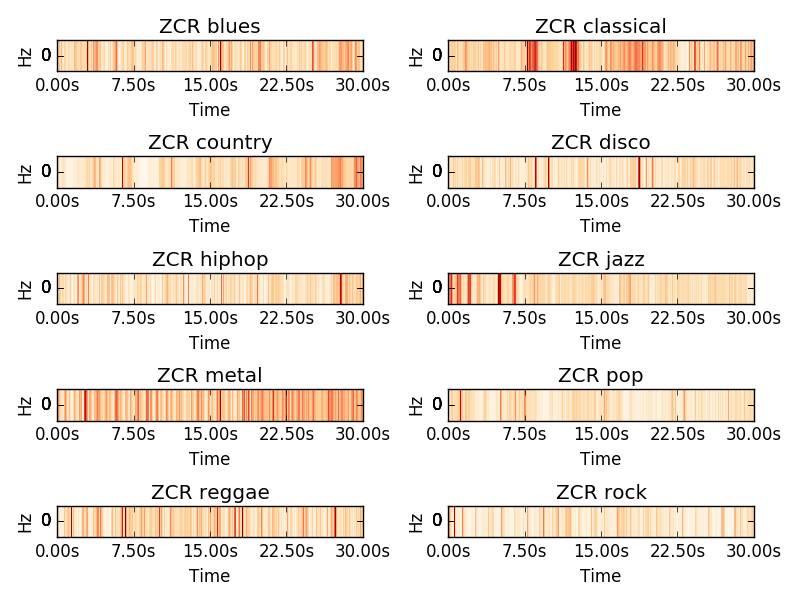
\includegraphics[width=\columnwidth]{ZCR_fig}
We can clearly see that different genres have different zero crossing rate distributions.
\subsection{Spectral Centroid}
The spectral centroid is a measure used in digital signal processing to characterise a spectrum. It indicates where the "center of mass" of the spectrum is. Perceptually, it has a robust connection with the impression of "brightness" of a sound.\cite{wiki}\par
It is calculated as the weighted mean of the frequencies present in the signal, determined using a Fourier transform, with their magnitudes as the weights:
\begin{equation}
    Centroid=\frac{\sum_{n=0}^{N-1}f(n)x(n)}{\sum_{n=0}^{N-1}x(n)}
\end{equation}
Spectral Centroid distribution for different genre files is given in following figure.\\
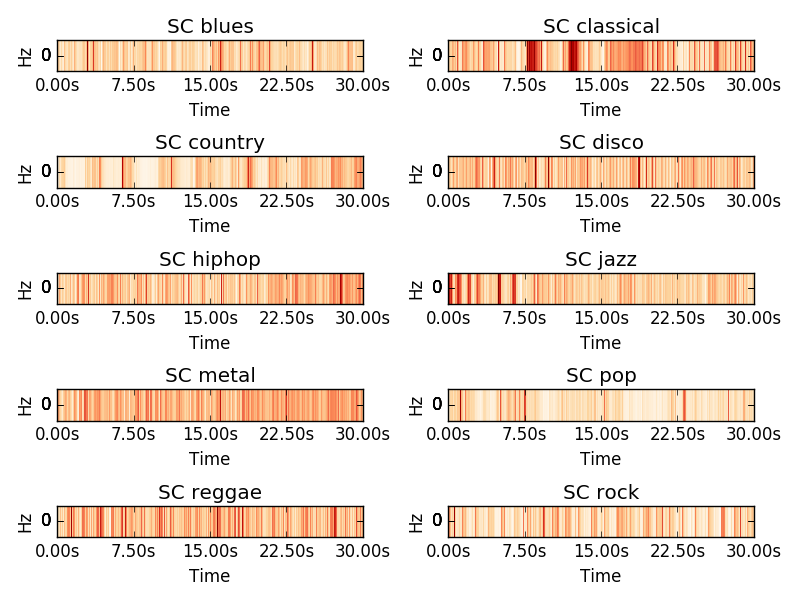
\includegraphics[width=\columnwidth]{SC_fig}
\subsection{Spectral Bandwidth}
Spectral Bandwidth is the Wavelength interval in which a radiated spectral quantity is not less than half its maximum value.
Spectral Bandwidth distribution for different genre files is given in following figure.\\
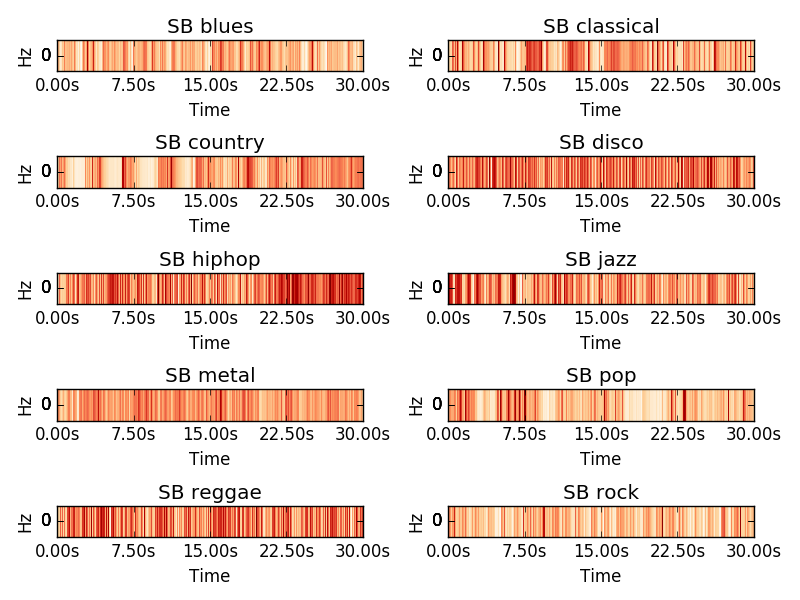
\includegraphics[width=\columnwidth]{SB_fig}
\subsection{Spectral Contrast}
Spectral contrast is defined as the decibel difference between peaks and valleys in the spectrum\cite{contrast}.
Spectral contrast distribution for different genre files is given in following figure.\\
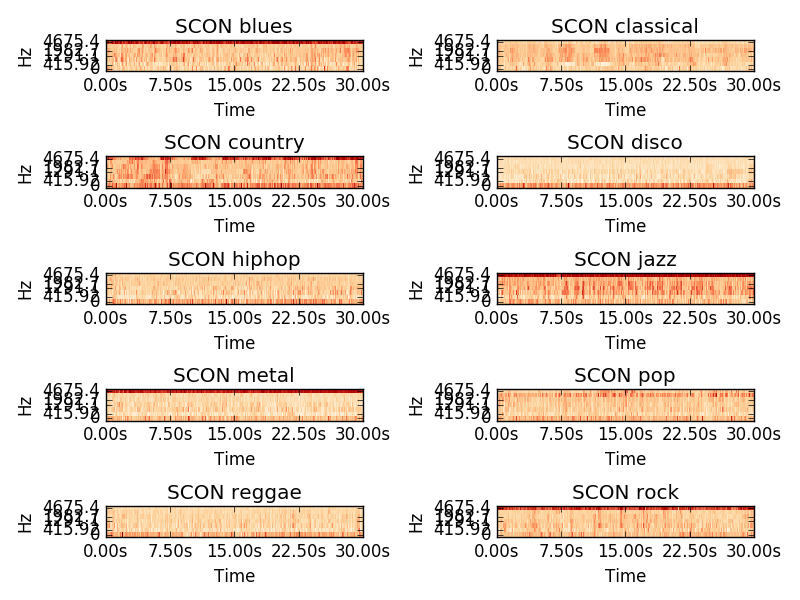
\includegraphics[width=\columnwidth]{SCON_fig}
\subsection{Spectral Rolloff}
Spectral Rolloff is a measure of the amount of the right-skewedness of the power spectrum. The spectral rolloff point is the fraction of bins in the power spectrum at which 85\% of the power is at lower frequencies\cite{jaudio}.
Spectral Rolloff distribution for different genre files is given in following figure.\\
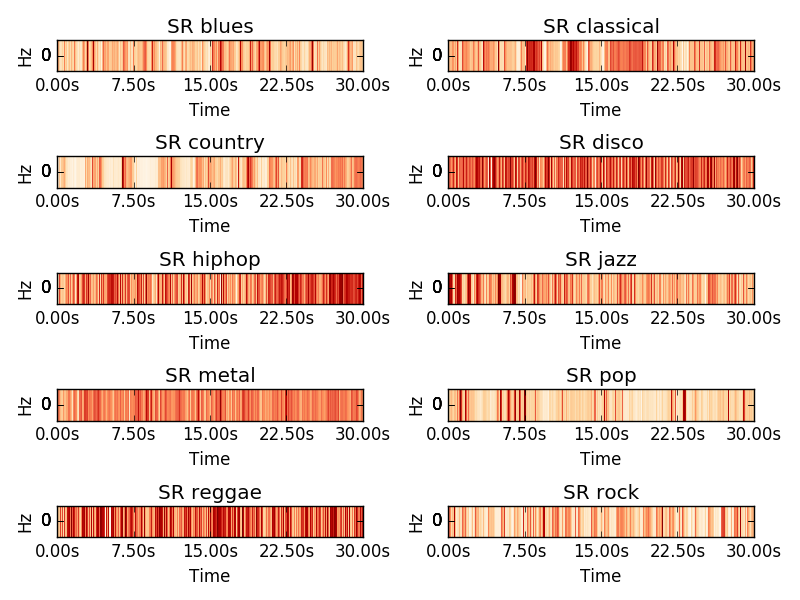
\includegraphics[width=\columnwidth]{SR_fig}
\subsection{Chroma Vector}
Chroma features are an interesting and powerful representation for music audio in which the entire spectrum is projected onto 12 bins representing the 12 distinct semitones (or chroma) of the musical octave. The term chroma closely relates to the twelve different pitch classes. Harmonic pitch class profiles (HPCP) is a group of features that a computer program extracts from an audio signal, based on a pitch class profile—a descriptor proposed in the context of a chord recognition system. Often, the twelve pitch spelling attributes are also referred to as chroma and the HPCP features are closely related to what is called chroma features or chromagrams\cite{wiki}.
Chroma Vector distribution for different genre files is given in following figure. From these image representations, this feature looks more promising than others for genre classification.\\
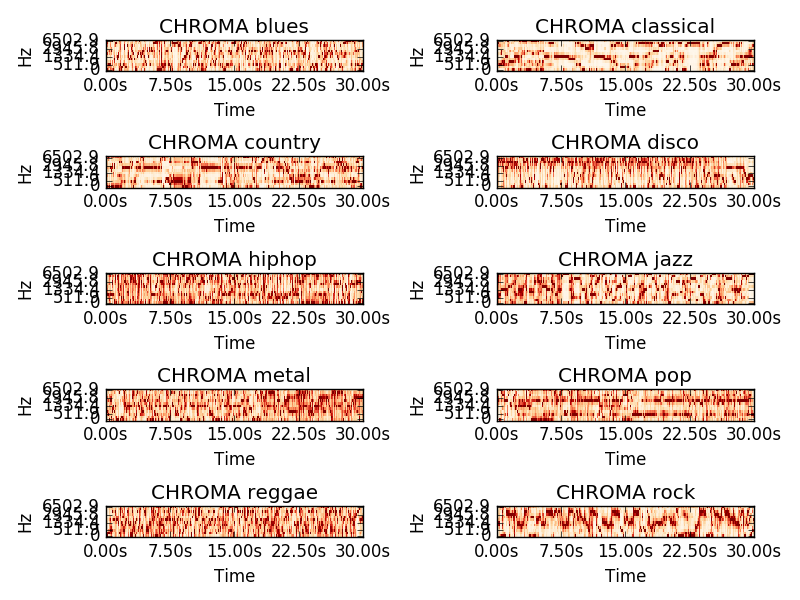
\includegraphics[width=\columnwidth]{CHROMA_fig}
\subsection{MFCC}
MFCC, Mel-Frequency Cepstral Co-efficients, a representation of the short-term power spectrum of a sound, based on a linear cosine transform of a log power spectrum on a nonlinear mel scale of frequency\cite{wiki}.
MFCC vector distribution for different genre files is given in following figure.\\
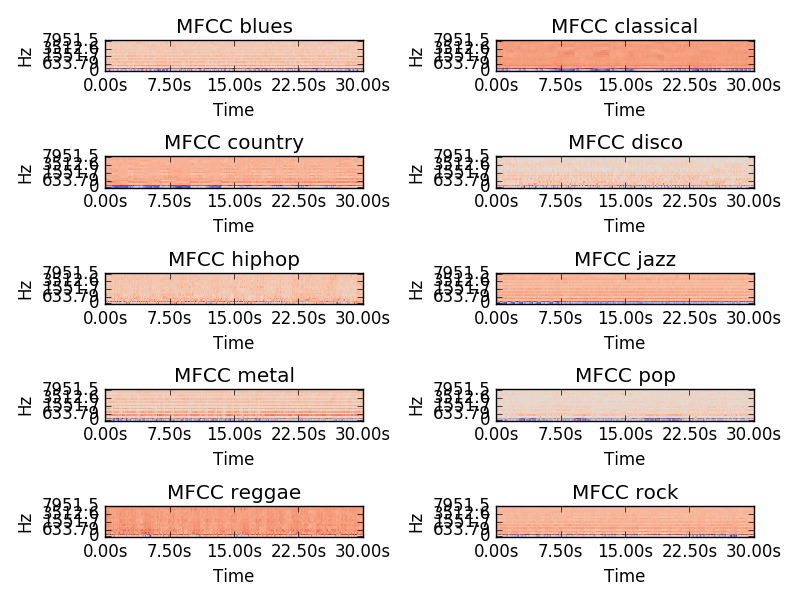
\includegraphics[width=\columnwidth]{MFCC_fig}
% An example of a floating figure using the graphicx package.
% Note that \label must occur AFTER (or within) \caption.
% For figures, \caption should occur after the \includegraphics.
% Note that IEEEtran v1.7 and later has special internal code that
% is designed to preserve the operation of \label within \caption
% even when the captionsoff option is in effect. However, because
% of issues like this, it may be the safest practice to put all your
% \label just after \caption rather than within \caption{}.
%
% Reminder: the "draftcls" or "draftclsnofoot", not "draft", class
% option should be used if it is desired that the figures are to be
% displayed while in draft mode.
%
%\begin{figure}[!t]
%\centering
%\includegraphics[width=2.5in]{myfigure}
% where an .eps filename suffix will be assumed under latex,
% and a .pdf suffix will be assumed for pdflatex; or what has been declared
% via \DeclareGraphicsExtensions.
%\caption{Simulation results for the network.}
%\label{fig_sim}
%\end{figure}

% Note that the IEEE typically puts floats only at the top, even when this
% results in a large percentage of a column being occupied by floats.


% An example of a double column floating figure using two subfigures.
% (The subfig.sty package must be loaded for this to work.)
% The subfigure \label commands are set within each subfloat command,
% and the \label for the overall figure must come after \caption.
% \hfil is used as a separator to get equal spacing.
% Watch out that the combined width of all the subfigures on a
% line do not exceed the text width or a line break will occur.
%
%\begin{figure*}[!t]
%\centering
%\subfloat[Case I]{\includegraphics[width=2.5in]{box}%
%\label{fig_first_case}}
%\hfil
%\subfloat[Case II]{\includegraphics[width=2.5in]{box}%
%\label{fig_second_case}}
%\caption{Simulation results for the network.}
%\label{fig_sim}
%\end{figure*}
%
% Note that often IEEE papers with subfigures do not employ subfigure
% captions (using the optional argument to \subfloat[]), but instead will
% reference/describe all of them (a), (b), etc., within the main caption.
% Be aware that for subfig.sty to generate the (a), (b), etc., subfigure
% labels, the optional argument to \subfloat must be present. If a
% subcaption is not desired, just leave its contents blank,
% e.g., \subfloat[].


% An example of a floating table. Note that, for IEEE style tables, the
% \caption command should come BEFORE the table and, given that table
% captions serve much like titles, are usually capitalized except for words
% such as a, an, and, as, at, but, by, for, in, nor, of, on, or, the, to
% and up, which are usually not capitalized unless they are the first or
% last word of the caption. Table text will default to \footnotesize as
% the IEEE normally uses this smaller font for tables.
% The \label must come after \caption as always.
%
%\begin{table}[!t]
%% increase table row spacing, adjust to taste
%\renewcommand{\arraystretch}{1.3}
% if using array.sty, it might be a good idea to tweak the value of
% \extrarowheight as needed to properly center the text within the cells
%\caption{An Example of a Table}
%\label{table_example}
%\centering
%% Some packages, such as MDW tools, offer better commands for making tables
%% than the plain LaTeX2e tabular which is used here.
%\begin{tabular}{|c||c|}
%\hline
%One & Two\\
%\hline
%Three & Four\\
%\hline
%\end{tabular}
%\end{table}


% Note that the IEEE does not put floats in the very first column
% - or typically anywhere on the first page for that matter. Also,
% in-text middle ("here") positioning is typically not used, but it
% is allowed and encouraged for Computer Society conferences (but
% not Computer Society journals). Most IEEE journals/conferences use
% top floats exclusively.
% Note that, LaTeX2e, unlike IEEE journals/conferences, places
% footnotes above bottom floats. This can be corrected via the
% \fnbelowfloat command of the stfloats package.


\section{Data preprocessing pipleline}
\label{sec:Data preprocessing}
We used Librosa an open source software framework for python for music data analysis. It also provides basic building blocks necessary to create music retrieval systems. We downloaded GTZAN genre classification dataset popularly used for musical research purpose for our project. It contains 1000 audio tracks each 30 seconds long. There are 10 genres represented each containing 100 tracks. All tracks are 22050 Hz Mono 16-bit audio files in .au format.

We wrote a python script which reads audio files of 100 songs per genre , extract all features and saves in a sqlite database. Once feature vectors are stored, multiple models
can be trained using combination of feature vectors. We further introduced custom matrix representation for each song which represents music feature mean vectors and covariances
of those features as 1-D vector, effectively modelling features as Multi-variate Guassian distribution. Lastly, we applied different supervised learning algorithms
using the reduced mean vector and covariance matrix as the features for each song to train on.

** picture of song broken into feature vector


Given a piece of music, each section of song(20 msec) is transformed into a vector with N dimensions and hence complete song can be transfomed into a feature matrix of N rows
and M columns where M = number of frames.

\section{Classification}
Once the feature vectors were obtained, we trained classifiers on diffrent set of feature vectors. We divided the dataset in 67\% - 33\% ratio for training and testing respectively. Feature selection is done manually by hit and trial method. Following were the different classifiers used:

\begin{enumerate}
  \item Multi Label K Nearest neighbour
  \item One-Vs-All approach with SVM
  \item Neural Network
  \item Non-Linear SVM
  \item Logistic Regression
  \item AdaBoost
  \item Bagging Classifier
\end{enumerate}


\subsection{Multi Label K Nearest Neighbour}
\label{sub:Multi Label K Nearest Neighbour}

Intutively, Music belongs to one genre should share same audio features. If we consider audio featuers as N dimensional vector then music belongs to one genre should be close to each other. This is similar to the idea behind multi-Label KNN algorithm in which it utilizes audio feature information of a music's k-nearest neighbour to infer its genres. We used above KL divergence measure (described below) for calculating similarity between two songs.

Consider $ p(x) $ and $ q(x) $ to be two song multivariate guassian distributions obtained from feature extraction. Then we have the following:

$$ 2KL(p||q) = \log{\left(\frac{\sum\nolimits_q}{\sum\nolimits_p}\right)} + Tr\left(\sum\nolimits_q^{-1}\sum\nolimits_p\right) $$

$$    + {\left(\mu_p - \mu_q\right)}^{T}\sum\nolimits_q^{-1}(\mu_p - \mu_q) - d $$


Since, KL divergence is not symmetric but the distance should be symmetric, Hence we used following similarity measure:
$$ {D}_{KL} =  KL\left(p||q\right) + KL\left(q||p\right) $$

Here we experimented with multiple values of K and found out that K=33 yields the best output.

\subsection{One vs All approach with SVM}
\label{sub:One vs All approach with SVM}

Also known as OVR (One vs Rest) multi class strategy. For each classifier, the class is fitted against all other classes. In addition to its computationally efficency only $n_classes$ classifiers are needed, one advantage of this approach is interpretability.

 We experimented with different cost penalties (1e-5 to 1e+5), loss functions (hinge and squared hinge) and penalty (L1 and L2) and observed that combination of L2 regularized hinge loss with C=100 yields the best result.

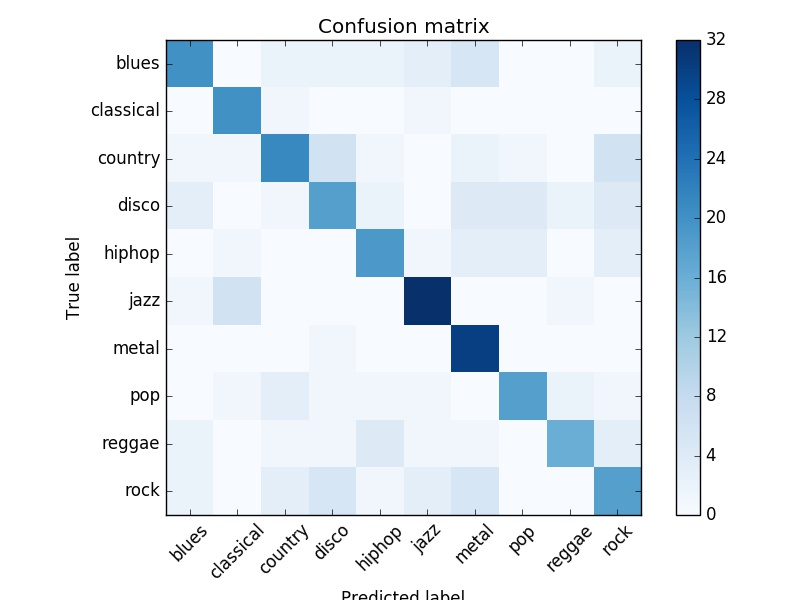
\includegraphics[width=\columnwidth]{LINEARSVC}

\subsection{Neural Network}
\label{sub:Neural Network}
In order to train the neural network data set was first normalized. Normalization implies that all feature values from dataset should have zero mean and unit standard deviation.

$$ X_n = \frac{X_n - \mu}{\sigma}$$

where $\mu$ is mean feature value and $ \sigma $ is standard deviation.

We trained neural network with 10\% of training instances as validation set which is the used to tune model parameters. We built a model with two hidden layer (10, 5), input layer size (256) and output layer size(10). We chose activation function as sigmoid function which gives us smooth non-linear function and cost function with regularization.


We also attempted to utilize PCA to reduce the dimension of input data but didn't improve our accuracy much.

Confusion matrix for ANN is given below.

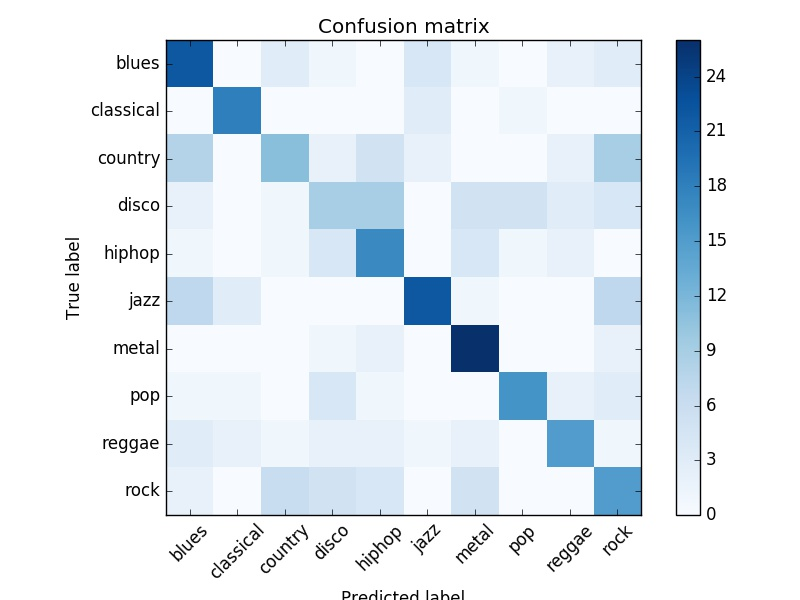
\includegraphics[width=\columnwidth]{ANN}
\subsection{Non-Linear SVM}
\label{subs:Non-Linear SVM}
Same as with Neural network, we first normalized the data and then feed it into SVM. SVMs are based on two properties: margin maximization (which allows for a good generalization of the classifier) and nonlinear transformation of the feature space with kernels(as data set is more easily seperable in high dimensional feature space).


We used Python scikit package to implement Non-linear SVM algorithm. It implements \"One-against-one\" approach (Knerr et. al 1990) for multiclass classification. if $n_class$ is the number of classes, then $n_class * (n_class - 1 ) / 2$ classifiers are constructed and each one trains data from two classes.

Confusion matrix for SVM is given below.
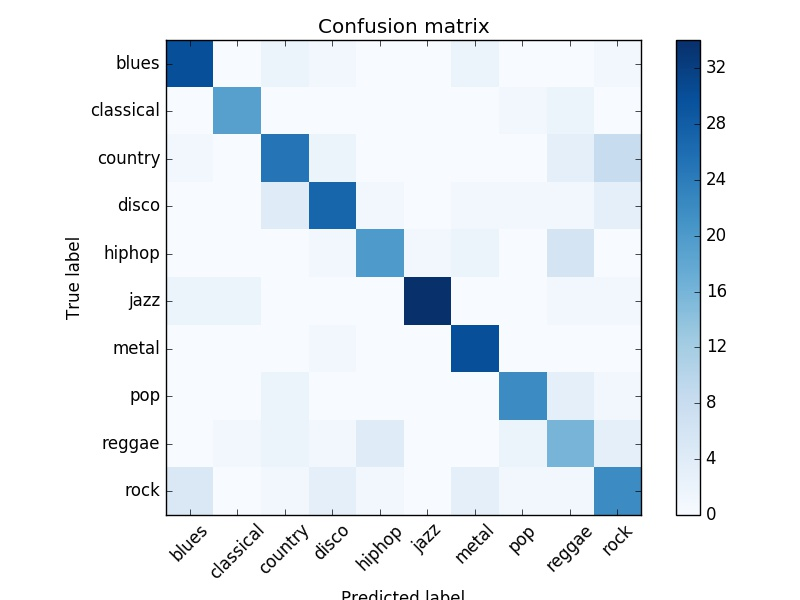
\includegraphics[width=\columnwidth]{SVM}
\subsection{Logistics Regression}
\label{sec:Logistics Regression}
It is again implemented using One-vs-rest scheme. We used regularized logistics regression with lbfgs solver. LBFGS solver works with L2 regularization. where best hyperparameter is selected by cross-validator StratifiedKFold mechanism.
Confusion matrix for Logistic Regression is given below.
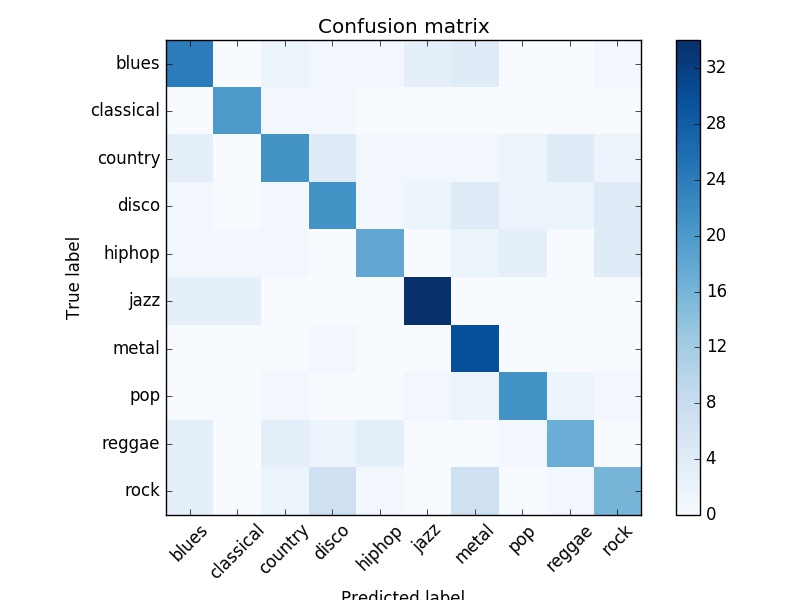
\includegraphics[width=\columnwidth]{LOGISTIC}


\subsection{AdaBoost}
\label{sub:AdaBoost Classification}
We used Adaboost algorithm to fit a sequence of weak learners on repeatedly modified versions of data. We experimented it with number of esimtaros and $learning_rate$ parameter. $n_estimator$ controls the number of iterations on models and $learning_rate$ controls the contribution of weak learners in final combination.

Here we experimented it with SVM as base estimator for adaboost and observed good classification results.
Confusion matrix for AdaBoost is given below.
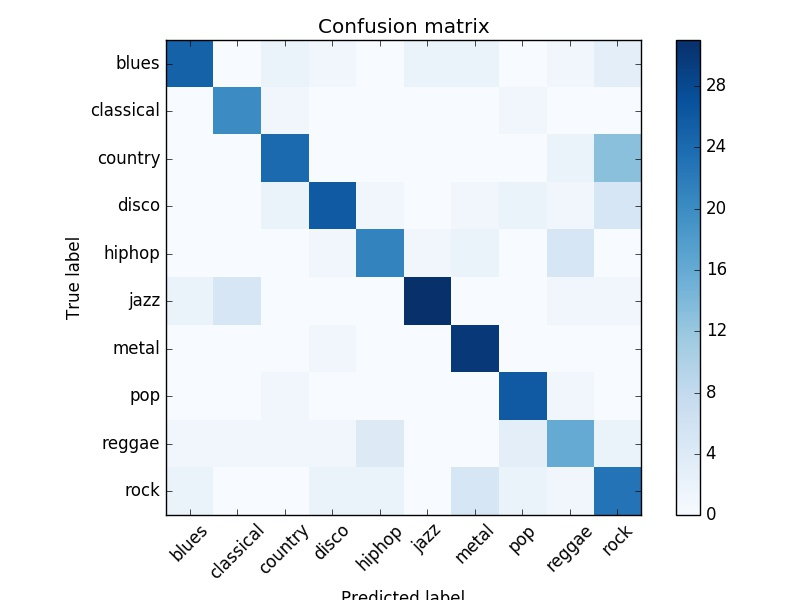
\includegraphics[width=\columnwidth]{ADABOOST}

\subsection{Bagging Classifier}
\label{sub:Baagging Classification}
We have also experimented on Bagging classifiers which fits base classifier each on random subsets of the original dataset and then aggregate the individual predictions(either by voting or by averaging) to form a final prediction. Such a meta-estimator is very useful in reducing the variance of base estimator by introducing randomization into its construction procedure and then making ensemble out of it.

Here we experimented it with SVM as base estimator as bagging classifier with varying number of model estimators.
Confusion matrix for Bagging classifier is given below.
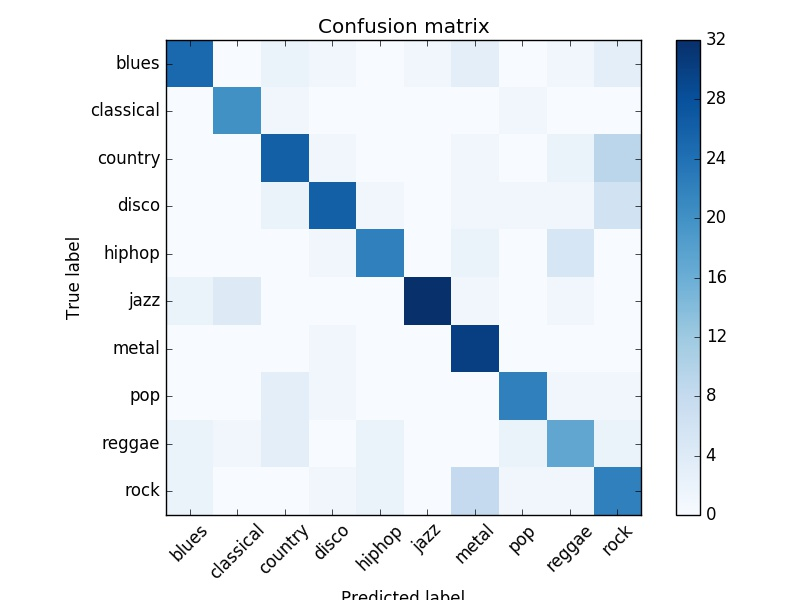
\includegraphics[width=\columnwidth]{BAGGING}

\section{Parameter Learning}
\label{sec:Results}

Hyperparameters of our classifiers are learnt based on the performance on validation set. Here we are showing parameter learning technique to Non-linear SVM classifier. We can clearly see in following figure that C=100 is optimal value for SVM parameter:

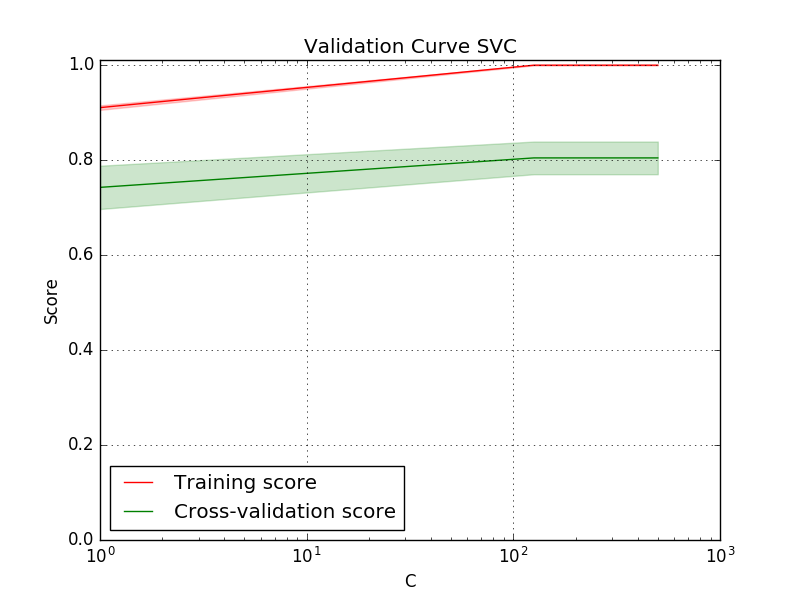
\includegraphics[width=\columnwidth]{validation}
\section{Overfitting Analysis}
To validate our SVM model does not suffer from bias/variance error, we applied learning curve analysis, which shows the training score is much greater than the validation score. Adding more training samples will most likely increase generalization. This proves that our model does not suffer form any bias vairance errors. 

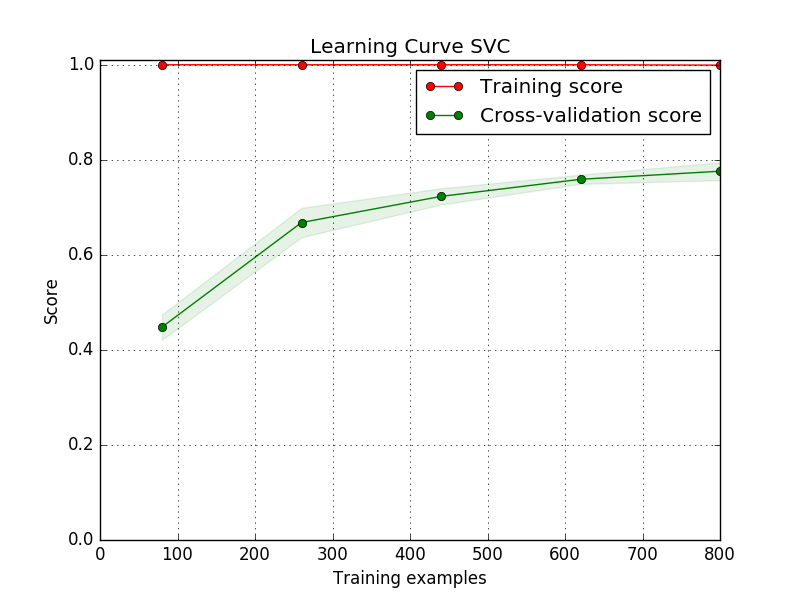
\includegraphics[width=\columnwidth]{learning}
\section{Classification Metrics}
Classification accuracy varied between the different machine learning techniques and genres. We got best accuracy with SVM classifier closed to 74\% accuracy. Reggae and Rock were difficult ones to classify whereas jazz achieved highest classification score. Here are some confusion matrix results for different classifiers. 
\subsection{Precision}
The precision is the ratio $\frac{tp}{tp + fp}$ where tp is the number of true positives and fp the number of false positives. The precision is intuitively the ability of the classifier not to label as positive a sample that is negative.
Below is the confusion matrix for precision values for different classifiers against different genres:

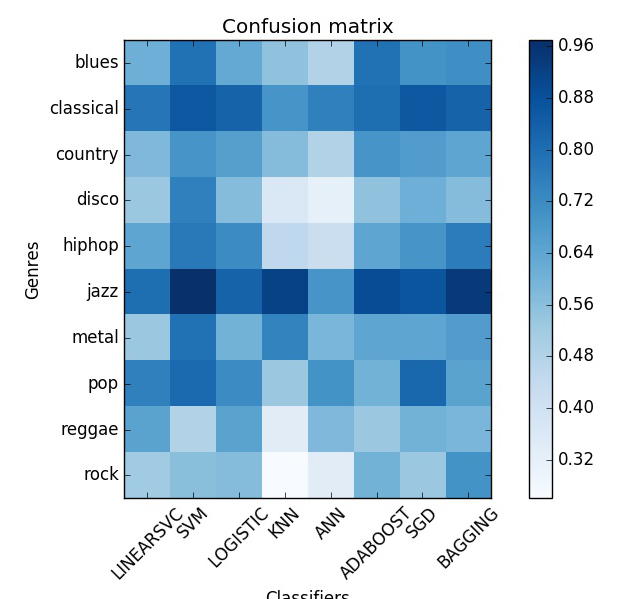
\includegraphics[width=\columnwidth]{precision}
We can clearly see that Jazz genre is having highest precision for almost all classifiers. Classical genre seems second best and consistent precision values for all classifiers. Rock seems to have low precision consistenly, because it is often confused as Metal, as can be seen from true label axis of Rock genre in Confusion matrices of diffrent classifiers.
\subsection{Recall}
The recall is the ratio $\frac{tp}{tp + fn}$ where tp is the number of true positives and fn the number of false negatives. The recall is intuitively the ability of the classifier to find all the positive samples.
Below is the confusion matrix for Recall values for different classifiers against different genres:

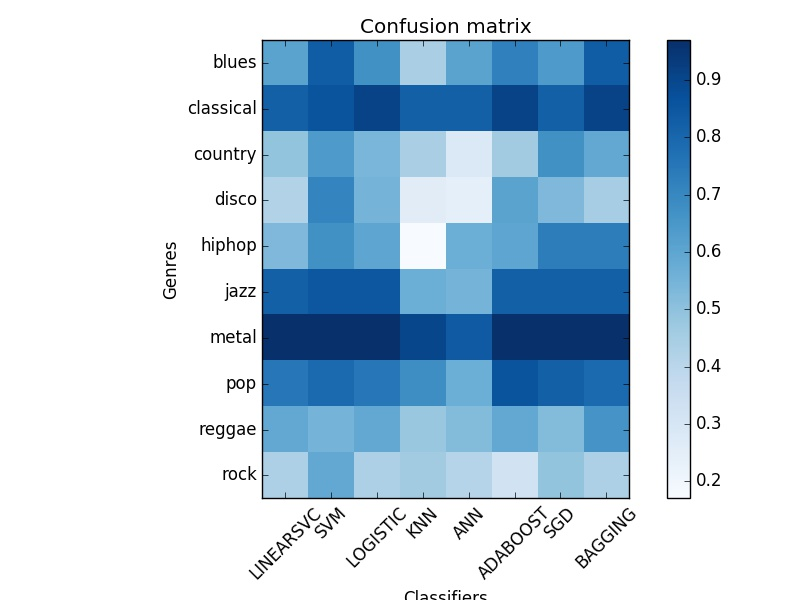
\includegraphics[width=\columnwidth]{recall}
Metal genre is having the highest recall among all classifiers. We can clearly see in confusion matrix images of different classifiers that almost all true labels of Metal have been classified as Metal. That's why the recall is high for Metal.
\subsection{F1 Score}
F1 score is harmonic mean of precision and recall values.
\begin{equation}
    F1=2 \cdot\frac{precision\cdot recall}{precision + recall}
\end{equation}
Below is the confusion matrix for F1 values for different classifiers against different genres:

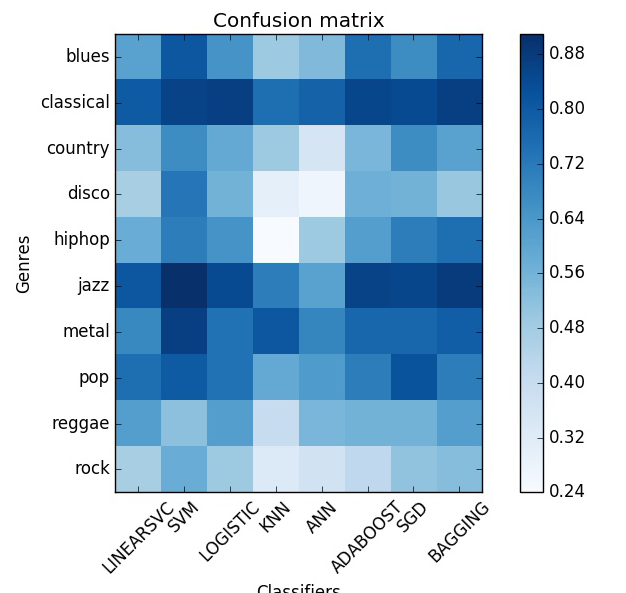
\includegraphics[width=\columnwidth]{f1score}

\section{Conclusion}
The conclusion goes here.



% conference papers do not normally have an appendix


% use section* for acknowledgment
\section*{Acknowledgment}


The authors would like to thank...





% trigger a \newpage just before the given reference
% number - used to balance the columns on the last page
% adjust value as needed - may need to be readjusted if
% the document is modified later
%\IEEEtriggeratref{8}
% The "triggered" command can be changed if desired:
%\IEEEtriggercmd{\enlargethispage{-5in}}

% references section

% can use a bibliography generated by BibTeX as a .bbl file
% BibTeX documentation can be easily obtained at:
% http://mirror.ctan.org/biblio/bibtex/contrib/doc/
% The IEEEtran BibTeX style support page is at:
% http://www.michaelshell.org/tex/ieeetran/bibtex/
%\bibliographystyle{IEEEtran}
% argument is your BibTeX string definitions and bibliography database(s)
%\bibliography{IEEEabrv,../bib/paper}
%
% <OR> manually copy in the resultant .bbl file
% set second argument of \begin to the number of references
% (used to reserve space for the reference number labels box)
\begin{thebibliography}{1}

\bibitem{gtzan}
    G. Tzanetakis and P. Cook, \emph{Musical genre classification of audio signals}.\hskip 1em IEEE Transactions on Audio and Speech Processing, 2002.
\bibitem{michael}
    Michael Haggblade, Yang Hong and Kenny Kao, \emph{Music Genre Classification}.\\ \url{http://cs229.stanford.edu/proj2011/HaggbladeHongKao-MusicGenreClassification.pdf}.
\bibitem{bob}
    Bob L. Sturm, \emph{An Analysis of the GTZAN Music Genre Dataset}. \hskip 1em MIRUM 2012.
\bibitem{wiki}
    \url{http://www.wikipedia.com}
\bibitem{base}
    Ioannis Panagakis, Emmanouil Benetos, and Constantine Kotropoulos, \emph{Music genre classification: a multilinear approach}. \hskip 1em ISMIR 2008.
\bibitem{zu}
    Fu, A., Lu, G., Ting, K.M., Zhang, D. \emph{A Survey of Audio-Based Music Classification and Annotation}. \hskip 1em IEEE transactions on multimedia 2010.
\bibitem{contrast}
    Jun Yang, Fa-Long Luo, Arye Nehorai. \emph{Spectral contrast enhancement: Algorithms and comparisons}. \hskip 1em Speech Communication - Special issue on speech processing for hearing aids, Vol 39, 2003.
\bibitem{jaudio}
    \url{http://jaudio.sourceforge.net/jaudio10/features/spectralrolloffpoint.html}
\end{thebibliography}




% that's all folks
\end{document}
